\documentclass[proceed]{article}
\usepackage{amsmath}
\usepackage{amsfonts}
\usepackage{multicol} \usepackage{fancyheadings} \usepackage{pdfpages}
\setlength{\emergencystretch}{10em}

\newtheorem{theorem}{Theorem}[section]
\newtheorem{lemma}[theorem]{Lemma}
\newtheorem{proposition}[theorem]{Proposition}
\newtheorem{corollary}[theorem]{Corollary}
 
\newenvironment{proof}[1][Proof]{\begin{trivlist}
\item[\hskip \labelsep {\bfseries #1}]}{\end{trivlist}}
\newenvironment{definition}[1][Definition]{\begin{trivlist}
\item[\hskip \labelsep {\bfseries #1}]}{\end{trivlist}}
\newenvironment{example}[1][Example]{\begin{trivlist}
\item[\hskip \labelsep {\bfseries #1}]}{\end{trivlist}}
\newenvironment{remark}[1][Remark]{\begin{trivlist}
\item[\hskip \labelsep {\bfseries #1}]}{\end{trivlist}}

\DeclareMathOperator*{\Exp}{\mathbb{E}}
\DeclareMathOperator*{\Prob}{\mathbf{P}}


\title{Qualitative Probabilistic Programming}
\author {}
\begin{document}

  \maketitle

  \begin{abstract}
    In probabilistic programs, sometimes it is difficult to specify the correct
    parameterized family of distributions.  We explore an extension to
    probabilistic programming languages that allows programmers to mark some
    distributions as unspecified.  Then, we can fill in the distribution with
    some family and infer parameters.
  \end{abstract}

  \section{Introduction}

  By separating model specification and inference, probabilistic programming 
  has made it easier for non-experts to implement and use probabilistic models.
  Practitioners frequently have strong intuitions about the {\em structure}
  of their domain knowledge, such as which latent variables exist and what
  their causal relations are, and probabilistic programming allows them to encode
  this knowledge. However, it also requires them to specify the specific parametric
  shape  and parameterization of any distributions used, and intuitions tend to
  be much less precise there.
  We present Quipp, a system that does {\em not} require such specification;
  instead, random variables and random functions can be left undefined
  and will automatically be filled in under maximum entropy assumptions
  based on their types and available datasets.
  
  Our formalism can concisely express a wide variety of models that machine
  learning practitioners care about, and we provide an expectation
  maximization algorithm that can learn the parameters for many of
  these models with reasonable efficiency. This system makes it easy
  for non-experts to encode their beliefs about the data and to get
  predictions based on as few additional assumptions as possible.
  
  % This feature has multiple advantages.  First, it is easier to write
  % models without knowing about the class of models being used.  This should
  % make probabliistic programming more accessible to non-experts.  Secondly,
  % parameter inference is more efficient if specialized algorithms are used
  % rather than the generic algorithms used to infer other random variables
  % (such as Metropolis Hastings).

  % We define an example probabilistic programming language with this feature
  % (Quipp) and show how it can be used to write machine learning models
  % concisely.

  In an ordinary probabilistic programming language (such as Church),
  it would be possible to treat parameters as random variables.  This
  would allow ordinary inference algorithms to infer parameters.  However,
  there are advantages of having unknown functions as a feature
  in the language.
  First, it is easier to
  write programs without knowing the details of different distributions.
  Second, specialized algorithms can be used to make parameter inference
  faster.

  % Inference in these models is performed using the expectation-maximization
  % algorithm, with alternating steps of inferring latent variables and optimizing
  % parameters.

  % - Motivation for Quipp
  %   - Explanation of "unknown functions"
  %   - Writing machine learning algorithms as probabilistic programs
  %   - Accessibility to non-experts
  %   - Comparison to existing probabilistic programming languages
  %     - In other languages, use random variables for parameters
  %     - Random variables slower because they are updated independently

  In the following, we first specify the syntax used to write Quipp programs,
  including the notation for unknown variables and functions.
  We describe the class of exponential family variables and functions that our system can learn,
  and present the expectation maximization algorithm used to learn them.
  We then demonstrate the expressiveness of our language, and the broad
  applicability of our algorithm, by writing some of the most common machine learning models
  in Quipp: clustering, factor analysis, a Hidden Markov model, Latent Dirichlet Allocation, and
  a neural net.
  
  \section{Syntax}

  Quipp is implemented as a Python library, so Quipp programs are written as Python programs that have access
  to special functions.  Here is an example of a Quipp program to perform clustering:


  \begin{verbatim}
  dim = 2
  nclusters = 3
  PointType = Vector(dim, Double)
  ClusterType = Categorical(nclusters)

  get_point = rand_function(ClusterType, PointType)

  def sample():
    cluster = uniform_categorical(nclusters)
    return (cluster, get_point(cluster))
  \end{verbatim}

  Notice that we declared two types (\texttt{PointType} and \texttt{ClusterType})
  and one random function \texttt{get\_point}).
  Type annotations are necessary for random functions.  The type
  \texttt{Vector(2, Double)} expresses the fact that the points are 2-dimensional,
  and the type \texttt{Categorical(3)} expresses the fact that there are 3
  possible clusters (so a cluster may be either 0, 1, or 2).  We assume that
  the disttribution over clusters is uniform, but we do not know the distribution
  of points in each cluster.
  We will fill in the
  \texttt{get\_point} function with a learned unknown linear function with noise.

  \section{Class of Distributions}

    For unknown functions, the class of random functions used is a kind
    of generalized linear model.  We assume that the result
    is distributed from some exponential family whose natural
    parameters are determined from the arguments.  We label
    some subset of the sufficient statistics as \emph{features}.  The natural
    parameters corresponding to non-features are constant, while natural
    parameters corresponding to features are determined as an affine
    function of the features of the arguments.

    Let $\psi_x$ be a matrix such that $\psi \phi(x)$ is a vector x of the
    features of $x$.  Then

    $$p_{\mathbf{N}}(y | x) = \exp(\psi(x)^T N \phi(y) - g(N^T \psi(X)))$$

    Given $(x, y)$ samples, parameter estimation to maximize log probability is a convex
    problem:

    \begin{align*}
      \log p_{\mathbf{N}}(y | x) = \psi(x)^T N \phi(y) - g(N^T \psi(X))
    \end{align*}
    since the log probability function is concave when $g$ is convex (as it is
    for any exponential family distribution).

    Therefore, it is possible to use Newton's method to optimize the parameters.

  \section{Inference}

    To perform inference of both latent variables and parameters, we first
    translate the program to a factor graph.  Next, we run the
    expectation maximization algorithm on this graph, iterating stages of
    estimating latent variables using Metropolis Hastings and parameter
    inference using Newton's method.

    In the factor graph, there are 2 types of variables: real numbers
    and categorical values.
    In Quipp, we have an additonal tuple type, which gets translated
    to multiple underlying variables in the factor graph.

    There are a few different types of factors:
    \begin{enumerate}
      \item Factors representing known distributions
      \item Factors representing unknown distribution
      \item Factors asserting that a value is equal to some constant
    \end{enumerate}

    How is inference in the factor graph performed?  We use the Metropolis Hastings
    algorithm, updating one node at a time.  To get a proposal for a given node,
    we approximate the local distribution using message passing (similar to
    in variational message passing).  Specifically, for each factor
    $f(x_1, x_2, ..., x_n)$ and each $1 \leq i \leq n$, we send a message
    to variable $x_i$ that approximates $x_i \mapsto f(x_1, x_2, ..., x_n)$.



  \section{Examples}

  \subsection{Clustering}
\begin{verbatim}
dim = 2
nclusters = 3

PointType = Vector(dim, Double)
ClusterType = Categorical(nclusters)

get_cluster = rand_function(ClusterType)
get_point = rand_function(ClusterType, PointType)

def sample():
  cluster = get_cluster()
  return (cluster, get_point(cluster))
\end{verbatim}

In this example, we cluster 2d points into 3 different clusters.  Given a cluster, the distribution for a point is some independent Gaussian distribution.  This is similar to fuzzy c-means clustering.

We randomly generated parameters for this example 100 times, and each time took 100 samples and then ran 10 EM iterations.  The accuracy is defined as the maximum percentage of points assigned to the correct cluster, for any permutation of clusters.  On average, accuracy increased in each EM iteration, as shown it this graph:

\begin{center}
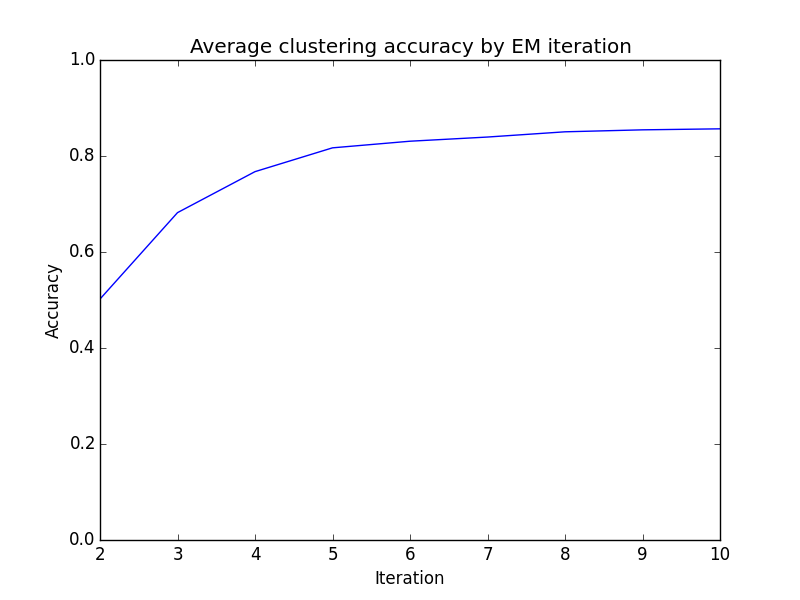
\includegraphics[scale=0.5]{cluster_accuracy.png}
\end{center}

\subsection{Naive Bayes}

\begin{verbatim}
nfeatures = 10
FeaturesType = Vector(nfeatures, Bool)

get_class = rand_function(Unit, Bool)

class_1_features = rand_function(Unit, FeaturesType)
class_2_features = rand_function(Unit, FeaturesType)

def sample():
  which_class = get_class()
  if which_class:
    features = class_1_features()
  else:
    features = class_2_features()
  return (which_class, features)
\end{verbatim}

The naive Bayes model is similar to the clustering model.  We have two classes and a feature
distribution for each.  Since each feature is boolean, we will learn
a different categorical distribution for each class.

(figure should show average classification accuracy)

  \subsection{Factor Analysis}

\begin{verbatim}
num_components = 3
point_dim = 5

ComponentsType = Vector(num_components, Double)
PointType = Vector(point_dim, Double)

get_point = rand_function(ComponentsType, PointType)

def sample():
  components = [normal(0, 1) for i in range(num_components)]
  return (comenents, get_point(components))
\end{verbatim}

The factor analysis model is very similar to the clustering model.  The main difference is that we replace the categorical \texttt{ClusterType} type with a vector type.  This results in the model attempting to find each point as an affine function of a vector of standard normal values.

(figure should show accuracy by EM iteration.  Accuracy can be measured by distances between different factor coefficients, when ordered according to some permutation)
  \subsection{Hidden Markov model}
\begin{verbatim}
num_states = 5
num_observations = 3
sequence_length = 10

StateType = Categorical(num_states)
ObsType = Categorical(num_observations)

trans_fun = rand_function(StateType, StateType)
obs_fun = rand_function(StateType, ObsType)

def sample():
  states = [uniform(num_states)]
  for i in range(sequence_length - 1):
    states.append(trans_fun(states[-1]))
  return (states, [obs_fun(s) for s in states])
\end{verbatim}

In this example, we use the unknown function \texttt{trans\_fun} for state transitions and \texttt{obs\_fun} for observations.  This means that we will learn both the state transitions and the observation distribution.


\subsection{Latent Dirichlet Allocation}

\begin{verbatim}
n_classes = 10
n_words = 100
n_words_per_document = 1000

ClassType = Categorical(n_classes)
WordType = Categorical(n_words)

class_to_word = rand_function(ClassType, WordType)

def sample():
    which_class = uniform_categorical(n_classes)
    words = [class_to_word(which_class) for i in range(n_words_per_document)]
    return (which_class, words)
\end{verbatim}

In this example, we use the unknown function \texttt{class\_to\_word} to map classes to word distributions.  Note that each column of the matrix of parameters for \texttt{class\_to\_word} will represent a categorical distribution over words, and there will be one column for each class.

(figure should show accuracy over time.  Accuracy can be measured as distance between the learned categorical distributions, for some permutation of classes)

\subsection{Neural Network}

\begin{verbatim}
input_dim = 100
hidden_dim = 20
output_dim = 2

InputType = Categorical(input_dim)
HiddenType = Categorical(hidden_dim)
OutputType = Categorical(output_dim)

input_to_hidden = rand_function(InputType, HiddenType)
hidden_to_output = rand_function(HiddenType, OutputType)

def sample(input_layer):
  hidden_layer = input_to_hidden(input_layer)
  output_layer = hidden_to_output(hidden_layer)
  return ((), output_layer)
\end{verbatim}

\subsection{A more complex model}

TODO: come up with a more complex model.  Show how this model can be iteratively improved by adding information.  It would make sense for this to be some sort of data science type  



  \section{Discussion}

  - Comments about results
  - Future directions
    - Unbounded models
    - Recursive algebraic data types


\end{document}

